\section{Durchführung}
\label{sec:Durchführung}
\begin{figure}
    \centering
    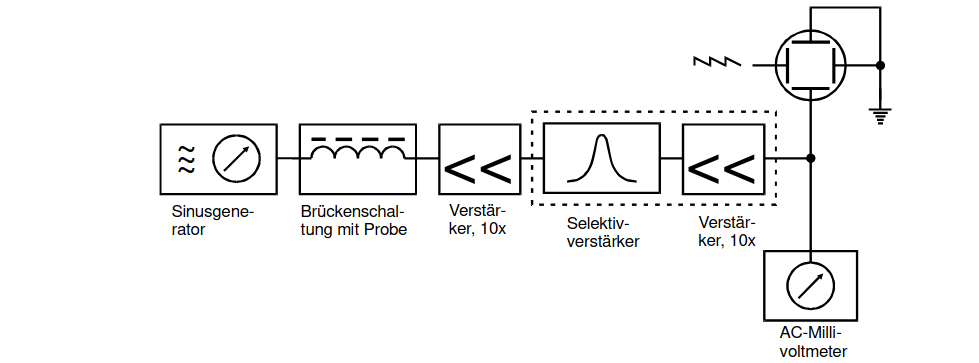
\includegraphics[width=\textwidth]{content/Aufbau.png}
    \caption{Schematischer Aufbau des Experimentes.\cite{anleitung}}
    \label{fig:schematisch}
\end{figure}
Der Versuchsaufbau ist nach \autoref{fig:schematisch} aufgebaut. 
Es wird eine Brückenschaltung, welche dem Schema von \autoref{fig:Brueckenschaltung} gleicht, mit einem Sinusgenerator gespeist.
Da an den Ausgangsklemmen der Brückenschaltung eine Störspannung vorhanden ist, welche die Brückenspannung überdecken würde, wird ein Selektivverstärker mit eingebauten Linearverstärkern benutzt.
Dieser lässt nur bestimmte Spannungen zu, welche dann von den AC-Millivoltmeter und dem Oszilloskop angezeigt werden. 

\subsection{Untersuchung des Selektivverstärkers}
Um die Filterkurve des Selektivverstärkers zu ermitteln, wird dieser mit einer konstanten Eingangsspannung $U_{\text{E}}$ gespeist.
Es wird eine Durchlassfrequenz $\nu_0$ zwischen $\num{20}$ und $\SI{40}{\kilo\hertz}$ eingestellt. 
Mit Hilfe eines Synthesizers werden verschiedene Frequenzen eingestellt und für diese jeweils die Ausgangsspannung $U_{\text{A}}$ gemessen.

\subsection{Messung der Suszeptibiltität}
Nun wird die Signalfrequenz des Sinusgenerators auf die Durchlassfrequenz des Selektivverstärkers gestellt.
Die Brückenschaltung wird abgeglichen und die Werte von $R_3$ sowie  $R_4$ werden notiert.
Anschließend wird die Probe in eine der Spulen eingesetzt und die Brückenspannung gemessen.
Danach wird die Brücke wieder abgeglichen und die neuen Werte von $R_3$ und $R_4$ notiert.
Dieses Vorgehen wird für jede der Proben drei Mal wiederholt.
Die Proben sind $\ce{Dy2O3}$ und $\ce{Gd2O3}$.